\section{Semantic Analysis}
\label{sec:implementation_semenaticAnalayis}
The second step in our compilation process is the semantic analysis of the input program. The analysis checks for any semantic errors in the code that can be detected before the next compilation step, the code generation. Our implementation of the semantic analysis differentiates between a declaration analysis and type checking. The declaration analysis is concerned with checking for errors related to the declaration of variables. For example, when a variable is used, it check whether it was declared previously or, when a variable is declared, the analysis ensure that the identifier is not in use in the current scope. In contrast, the type checking ensures that the type of a variable is consistent with the use of the variable. 

Both analyses are implemented as separate \texttt{Listeners}.
\todo{describe in \ref{sec:implementation_syntax_dataStructuresClasses}} 
This is done to separate both classes and give them concrete purposes while making the overall structure of the compiler more modular. In turn, since both analyses are implemented separately, they currently each require a traversal of the parse tree making the semantic analysis more inefficient. However, this can easily be addressed by writing a \texttt{Listener} that wraps both analyses, traverses the parse tree only once, and calls the corresponding function for each wrapped analysis.     

\subsection{Declaration Analysis}
\label{sec:implementation_declarationAnalayis}
The declaration analysis reports any errors that caused by the use of identifiers in invalid contexts; these are the use of an undeclared variable, the declaration of a variable in a context where it is already defined, and the use of a qubit in a code block which is guarded by itself.
\todo{Define when a code block is guarded by a qubit.}
Additionally, it also reports a warning when a variable is declared but never used.

For its analysis, the class creates a symbol table and adds any symbol that is declared. Further, is executes all other functions required for a valid analysis with the symbol table, like pushing scopes onto and popping them from the stack in the symbol table at the locations in the parse tree transversal where it is required. Before adding a symbol to the table, \ie every time the parse tree transversal exits a declaration, the \texttt{Listener} checks whether the identifier is already declared in the current context; if this is the case, the corresponding error is reported. Similarly, each time an identifier is referenced outside of a declaration, the analysis ensures that the variable is defined, otherwise it reports the corresponding error as well. Lastly, whenever a register rule is encountered in the transversal, the analysis not only checks that the variable is declared but also whether the current code block is guarded by the referenced register. If this is the case, the analysis reports an error. While the register parsing rule is only used for gate applications and if-statements and not for function calls such as \texttt{sizeof}, only performing the check the register rule cannot result in an invalid use of an identifier. This is the case because all function calls result in constant values and only refer to properties of a register, not the register itself; therefore, the compiled program will not have a reference to the register in the controlled context.\todo{Cannot check for all cases, some need to be at generation time}

While the symbol table suffices for reporting the previous errors, it does not track the usage of symbols. Therefore, it cannot be used for the unused symbol warning. For this analysis, the class contains a dictionary that maps a symbol to the number of references. Each time a symbol is added to the symbol table, the corresponding entry in the dictionary is initialized to zero. Then, for every reference to the symbol, its usage counter is incremented. At the end of the tree transversal, specifically when exiting the main code block, the analysis iterates over all entries in the dictionary and reports a warning whenever the usage counter is still $0$. However, there is an exception if an identifier is the underscore character so that it can be used as a throwaway variable, similar to other programming language.  

\subsection{Type Checking}
\label{sec:implementation_typeCheckingAnalayis}
\begin{itemize}
    \item What does type checking do?
    \begin{itemize}
        \item checks the use of symbols
        \item ensure that they are used in a valid context
    \end{itemize}
    \item How is this accomplished?
    \begin{itemize}
        \item for each use of an identifier, the type of the symbol is checked
        \item Register only allows either register, and if index is given, cannot be qubit, any parameter type checking is skipped
        \item Identifier in factor rule can only either be loop iterator or constant symbol, because numeric value is required, in turn, eg register is not valid
        \item for gate application, all given registers are checked, is not register type error, composite gates allow registers, constant gates only qubits
        \item furthermore, number of arguments is checked against required
        \item if statement requires qubit or register with qubit access
        \item range is checked for valid range, can throw invalid range exception
        \item when leaving the gate rule, and an identifier is given, corresponding symbol needs to be a composite gate
        \item function allows for identifiers when using size of function, only allows registers
        \item 
    \end{itemize}
    \item Similar to declaration analysis, symbol table is used
    \item All declarations correctly add the symbols so that the info can be used to for the type checking, additionally the scopes are pushed  
\end{itemize}
Type checking is used to ensure that any use of a symbol occurs in a valid context for this symbol. For example, while a qubit symbol can be used as the argument for a gate application, it does not represent a classical numerical value and, therefore, cannot be used in the context of a factor. Similar to the declaration analysis, a symbol table is used and all symbols, that are declared while traversing the tree, are added to it. Additionally, the scopes are also pushed and popped according to the traversal to allow differently typed variables in independent scopes.

To check the use of a symbol, each grammar rule where an identifier can be used checks its type. To do this, each function gets the identifier string and retrieves the corresponding symbol information from the symbol table. In the case of the register rule, only register symbols are allowed. The 

\subsection{Error Handling}
\label{sec:implementation_semanticAnalayis_errorHandling}
Error handling is an essential part of both the semantic analysis and code generation phase of the compiler; without clear and informative error messages, debugging compilation error is both challenging and tedious. Therefore, our compiler contains a number of different compilation errors. All there errors inherit from an abstract compilation error class. 

The abstract compilation error class contains three different properties. The first property is the error type. Currently, there are two different error type possible in the compiler, a warning and a critical error. While a warning indicates an issue with the source program which can still be compiler, a critical error in the source code cannot be compiled and results in the abortion of the compilation progress. Secondly, the description property should hold a description of the error that can be used to inform the programmer what issue occurred. Lastly, the error context saves relevant information about the source code properties of the error; it is implemented as a \texttt{struct} that contains both the line and column index of the source code location of the error. The error context can be created either from the line and column directly, the token where the error occurred, or the parsing rule with which the error is associated. In many cases, the error context can be created when the error occurs. For example, if an undefined identifier error is found in the declaration analysis, the parser rule context is given an the error can easily be created from it. However, in other cases, error may be thrown at generation time and the corresponding parser rule context may no longer be know. Therefore, all symbol also contain the error context corresponding to their declaration. 

While the abstract compilation error class contains general properties that are required for all errors, each error may contain additional properties that are required to give a clear and informative description of the error. Since many error occur in reference to a specific identifiers, the compiler uses an additional abstract identifier error that contains a string property which holds the identifier. The invalid access, type, invalid size, redefine, and use of guard error are all identifier errors. While the undefined error is also related to an identifier, it holds a list of identifiers instead of just a single one. This is because it is also used for undefined identifiers in an expression, where multiple are possible. Since they are in the same context, \ie the same expression, they are accumulated into a single error to reduce the number of errors. Additionally, many error are related to an invalid argument or invalid number of arguments. In this case, the given argument or number of arguments is saved in the error object; this is the case for the invalid function arguments, invalid number of argument, invalid access, invalid range, and invalid size error. In some cases, the required arguments are apparent from other properties, \eg the invalid number of arguments error contains a gate interface which specifies the number of required arguments. In contrast, other error specifically contains the required number of arguments, as they are specified by other properties, \eg the invalid function argument. All the different errors, including their respective properties, are depicted in Fig.~\ref{fig:implementation_uml_errors}.

\begin{figure}[htp]
    \centering
    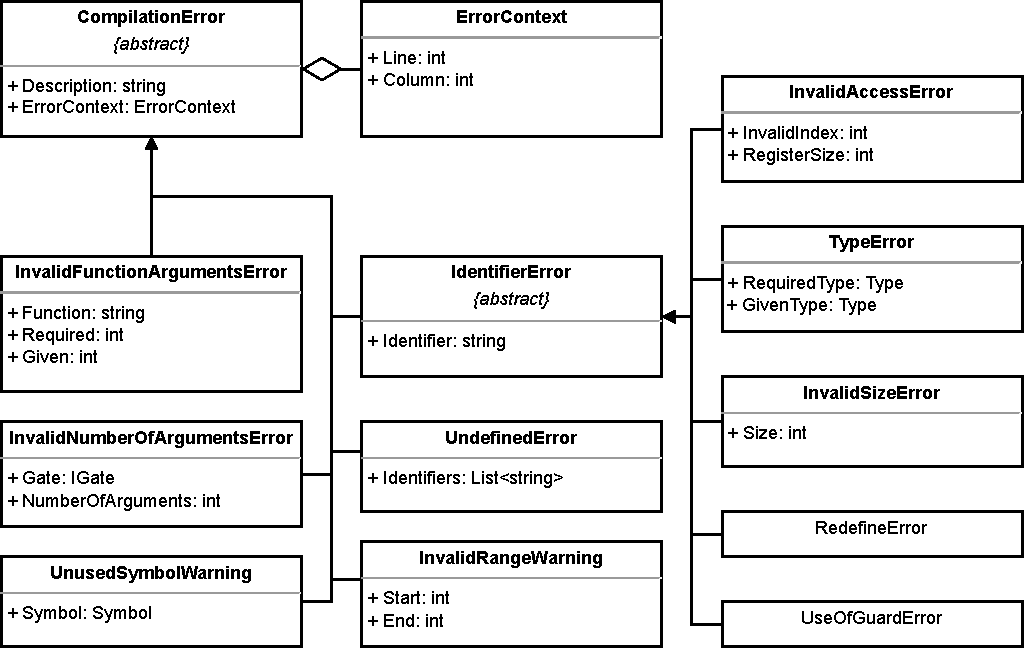
\includegraphics[width=.9\textwidth]{../figures/uml_errors.pdf}
    \caption{UML diagram of the different errors.}
    \label{fig:implementation_uml_errors}
\end{figure}

One advantage of a semantic analysis separate from the code generation is that, if an error is found, the semantic analysis can continue. For example, if an undefined identifier error occurs while generating code, the code generation can no longer continue as the identifier cannot be mapped to a symbol and, therefore, the information for the code generation is incomplete. However, a semantic analysis can continue as it does not need any more information about a symbol than its existence. In turn, while error in the code generation phase use typical error handling with exceptions that abort the tree traversal, the semantic analysis uses a custom error handler. Mainly, this error handler object consists of a list of compilation error and a report function that takes an error and adds it to the list. Additionally, the handler also contains properties that indicate whether it contains critical errors and two lists that return only the critical errors or warnings respectively. After the semantic analysis, the compiler will iterate over the errors in the handler in print them as either errors or warnings, depending on their error type.\unsure{Internal exceptions explained here?}